%%%%%%%%%%%%%%%%%%%%%%%%%%%%%%%%%%%%%%%%%%%
%%% DOCUMENT PREAMBLE %%%
\documentclass[12pt]{report}
\usepackage[italian]{babel}

\usepackage[normalem]{ulem}
\useunder{\uline}{\ul}{}
\usepackage{longtable}
\usepackage{url}
\usepackage{placeins}
\usepackage[utf8x]{inputenc}
\usepackage{amsmath}
\usepackage{graphicx}
\graphicspath{{images/}}
\usepackage{parskip}
\usepackage{fancyhdr}
\usepackage{vmargin}
\usepackage{nameref}
\setmarginsrb{3 cm}{2.5 cm}{3 cm}{2.5 cm}{1 cm}{1.5 cm}{1 cm}{1.5 cm}

\title{uCOM}								
% Title
\author{Mazzaglia Pietro}						
% Author

\makeatletter
\let\thetitle\@title
\let\theauthor\@author
\newcommand*{\currentname}{\@currentlabelname}
\makeatother

\pagestyle{fancy}
\fancyhf{}
\lhead{\thetitle}
\rhead{\currentname}
\cfoot{\thepage}


\begin{document}
	
	\huge \textbf{Elaborazione - Iterazione 1}
	
	\renewcommand{\thesection}{\arabic{section}}
	
	\normalsize
	
	%%%%%%%%%%%%%%%%%%%%%%%% PIANIFICAZIONE %%%%%%%%%%%%%%%%%%%%%%

	\section{Introduzione}
	
	Durante le diverse iterazioni della fase di elaborazione vengono raffinati gli elaborati abbozzati durante la fase di Ideazione e si procede all'analisi e alla progettazione del software. \\
	Durante ogni iterazione verrà inoltre implementata parte del prodotto finale, con i relativi test, per fornire al cliente versioni di prova del software corrette e funzionanti, seppure parziali.
	
	Gli obiettivi della prima iterazione sono:
	\begin{itemize}
		\item Analisi e progettazione, relativamente agli scenari dei casi d'uso \textit{UC4: Invia comunicazione} e \textit{UC9: Effettua accesso}
		\item Implementazione (parziale) degli scenari di successo dei casi d'uso, e dei relativi test
	\end{itemize}
	
	Sono stati scelti i casi d'uso citati, in quanto permettono di iniziare a sviluppare il nucleo del sistema \textit{uCOM}, di risolvere alcuni elementi ad alto rischio e di soddisfare alcuni tra i requisiti più importanti, tra cui sicurezza e affidabilità.
	
	\section{Pianificazione e gestione del progetto}
	
	Nella scelta degli obiettivi per questa iterazione sono stati organizzati i requisiti e le interazioni sulla base del rischio, della copertura e della criticità. 
	
	% Please add the following required packages to your document preamble:
	% \usepackage{graphicx}
	\begin{table}[!htb]
		\centering
		\resizebox{\textwidth}{!}{%
			\begin{tabular}{|l|l|l|}
				\hline
				\textbf{Priorità} & \textbf{Requisiti  (Casi d'uso o funzionalità)}                                                                          & \textbf{Commento}                                                                                                                                                                                                                                \\ \hline
				Alta              & \begin{tabular}[c]{@{}l@{}}\textbf{Invia comunicazione}\\ \\ Invia avviso\\ \\ Gestisce utente\\ \\ \textbf{Effettua accesso}\end{tabular} & \begin{tabular}[c]{@{}l@{}}\textbf{Nucleo della piattaforma, alta frequenza}\\ \\ Nucleo della piattaforma, alta frequenza\\ \\ Nucleo della piattaforma, sicurezza\\ \\ \textbf{Nucleo della piattaforma, sicurezza, coinvolta in tutte le funzioni}\end{tabular} \\ \hline
				Media             & \begin{tabular}[c]{@{}l@{}}Prenota pasto\\ \\ Richiede libro\end{tabular}                                                & \begin{tabular}[c]{@{}l@{}}Frequenza elevata e più parti interessate ma sostituibile\\ \\ Frequenza elevata e più parti interessate ma sostituibile\end{tabular}                                                                                 \\ \hline
				Bassa             & \begin{tabular}[c]{@{}l@{}}Iscrive a un corso\\ \\ Gestisce corso\\ \\ Gestisce iscrizione corso\end{tabular}            & \begin{tabular}[c]{@{}l@{}}Bassa frequenza e sostituibile\\ \\ Bassa frequenza e sostituibile\\ \\ Bassa frequenza e sostituibile \end{tabular}                                                                                                                                                \\ \hline
			\end{tabular}%
		}
	\end{table}
	
	\newpage
	
	\section{Modello dei casi d'uso}
	
	Seguono l'aggiornamento dell'\textit{UC4} con correzioni e precisazioni rispetto alla fase di Ideazione e la descrizione dettagliata dell'\textit{UC9}.
	
	Inoltre si presentano i \textit{Diagrammi di sequenza di sistema} relativi agli scenari di successo e i \textit{Contratti delle operazioni}.
	
	\subsection{UC4: Invia comunicazione}

	
	% Please add the following required packages to your document preamble:
	% \usepackage{longtable}
	% Note: It may be necessary to compile the document several times to get a multi-page table to line up properly
	\begin{longtable}[c]{|l|l|}
		\hline
		\textbf{Nome caso d'uso}                                                                          & UC4: Invia comunicazione                                                                           \\ \hline
		\endfirsthead
		%
		\endhead
		%
		\textbf{Portata}                                                                                  & Piattaforma uCOM                                                                                                                                                                                                                                                                                                                                                                                                                                                                                                                                                                                                                                                                                                                                                                                                                                                                                                                                                                                                                                                                                                                       \\ \hline
		\textbf{Livello}                                                                                  & Obiettivo utente                                                                                                                                                                                                                                                                                                                                                                                                                                                                                                                                                                                                                                                                                                                                                                                                                                                                                                                                                                                                                                                                                                                       \\ \hline
		\textbf{Attore primario}                                                                          & Studente                                                                                                                                                                                                                                                                                                                                                                                                                                                                                                                                                                                                                                                                                                                                                                                                                                                                                                                                                                                                                                                                                                                               \\ \hline
		\textbf{\begin{tabular}[c]{@{}l@{}}Parti interessate \\ e Interessi\end{tabular}}                 & \begin{tabular}[c]{@{}l@{}}\textit{Studente: }vuole inviare una comunicazione relativa\\ alla vita all'interno del Campus\\ \\ \textit{Amministrazione: }vuole potere ricevere la comunicazione\\  dello studente\\ \\ \textit{Direzione Campus:} vuole che la comunicazione \\ avvenga in maniera rapida, sicura e affidabile\end{tabular}                                                                                                                                                                                                                                                                                                                                                                                                                                                                                                                                                                                                                                                                                                                                                                                                                       \\ \hline
		\textbf{Pre-condizioni}                                                                           & Lo Studente possiede un account sulla piattaforma.                                                                                                                                                                                                                                                                                                                                                                                                                                                                                                                                                                                                                                                                                                                                                                                                                                                                                                                                                                                                                                                                                     \\ \hline
		\textbf{Garanzia di successo}                                                                     & Lo Studente ha ricevuto conferma dell'operazione.                                                                                                                                                                                                                                                                                                                                                                                                                                                                                                                                                                                                                                                                                                                                                                                                                                                                                                                                                                                                                                                                                      \\ \hline
		\textbf{\begin{tabular}[c]{@{}l@{}}Scenario principale \\ di successo\end{tabular}}               & \begin{tabular}[c]{@{}l@{}}1. Lo Studente effettua l'accesso\\ 2. Lo Studente avvia l'operazione di invio della comunicazione.\\ 3. Lo Studente inserisce oggetto e corpo della comunicazione.\\ 4. Lo Studente invia la comunicazione.\\ 5. Il Sistema elabora la comunicazione.\\ 6. Il Sistema conferma la riuscita dell'operazione.\end{tabular}                                                                                                                                                                                                                                                                                                                                                                                                                                                                                                                                                                                                                                                                                                                                                                                                 \\ \hline
		\textbf{Estensioni}                                                                               & \begin{tabular}[c]{@{}l@{}}*a. In qualsiasi momento.Il Sistema non è in grado di funzionare \\ correttamente in un dato momento.\\ \\  \quad   1) Il Sistema segnala l'impossibilità di eseguire l'azione.\\ \\  \quad   - Lo Studente riprova a eseguire l'azione dopo un certo periodo\\     di tempo.\\ \\  *b. In qualsiasi momento. Il Sistema entra in uno stato di errore\\ irrisolvibile.\\ \\  \quad   1) Il Sistema termina la sessione, perdendo i dati.\\ \\  \quad   - Lo Studente deve ricominciare l'operazione.\\ \\ *c. In qualsiasi momento. Lo Studente interrompe l'operazione. \\ \\ \quad 1)Il Sistema termina l'operazione. \\ \\ 3a. Lo Studente inserisce informazioni non valide.\\ \\  \quad   1) Il Sistema richiede nuova immissione dei dati allo Studente.\\ \\ 5a. Il Sistema invia il messaggio a un Servizio Esterno.\\ \\  \quad   1a) Il Servizio Esterno riceve correttamente il messaggio.\\  \\    \quad \quad     2) Il Sistema conferma la riuscita dell'operazione.\\ \\  \quad   1b) Il Servizio Esterno rigetta la richiesta.\\ \\    \quad \quad     - Il Sistema va in errore temporaneo.\\ \\   \quad \quad      - Lo Studente può ritentare l'operazione dopo un certo\\           periodo di tempo.\\ \\ 5b. Il Sistema gestisce internamente il messaggio.\end{tabular} \\ \hline
		\textbf{Requisiti speciali}                                                                       & \begin{tabular}[c]{@{}l@{}}- Lo Studente deve poter inserire le informazioni nella propria\\ lingua o nella lingua di comunicazione del Campus.\end{tabular}                                                                                                                                                                                                                                                                                                                                                                                                                                                                                                                                                                                                                                                                                                                                                                                                                                                                                                                                                                           \\ \hline
		\textbf{\begin{tabular}[c]{@{}l@{}}Elenco delle varianti \\ tecnologiche e dei dati\end{tabular}} & \begin{tabular}[c]{@{}l@{}}3) L'inserimento delle informazioni può avvenire attraverso\\ metodi d'input diversi, come tastiera e mouse o un touchscreen.\\ \\ 5) L'elaborazione di sistema può avvenire internamente o\\ esternamente alla piattaforma uCOM.\end{tabular}
		\\ \hline
		\textbf{Frequenza di ripetizione}                                                                 & quasi giornaliera                                                                                                                                                                                                                                                                                                                                                                                                                                                                                                                                                                                                                                                                                                                                                                                                                                                                                                                                                                                                                                                                                                                      \\ \hline
		\textbf{Varie}                                                                                    & \begin{tabular}[c]{@{}l@{}}Si potrebbe prevedere un sistema che permetta l'inserimento\\ offline e l'elaborazione non appena il servizio ritorna disponibile.\\ \\ Si potrebbe integrare il servizio esterno all'interno della\\ piattaforma, piuttosto che inviare esternamente il messaggio \\ per l'elaborazione.\\ \\ Il messaggio viene memorizzato dal Sistema se viene elaborato\\ esternamente?\\ \\ Si possono prevedere meccanismi di recupero dell'istanza in\\ caso di errori gravi. \\ \\ Si potrebbe prevedere l'aggiunta di allegati alla comunicazione.\end{tabular}                                                                                                                                                                                                                                                                                                                                                                                                                                                                                                                                                                                                                 \\ \hline
	\end{longtable}	

	\subsection{UC9: Effettua accesso}

	\begin{longtable}[c]{|l|l|}
		\hline
		\textbf{Nome caso d'uso}                                                                          & UC9: Effettua accesso                                                                                                                                                                                                                                                                                                                                                                                                      \\ \hline
		\endfirsthead
		%
		\endhead
		%
		\textbf{Portata}                                                                                  & Piattaforma uCOM                                                                                                                                                                                                                                                                                                                                                                                                           \\ \hline
		\textbf{Livello}                                                                                  & Sottofunzione                                                                                                                                                                                                                                                                                                                                                                                                              \\ \hline
		\textbf{Attore primario}                                                                          & Utente (Studente/Amministratore/System Admin)                                                                                                                                                                                                                                                                                                                                                                              \\ \hline
		\textbf{\begin{tabular}[c]{@{}l@{}}Parti interessate \\ e Interessi\end{tabular}}                 & \begin{tabular}[c]{@{}l@{}}Utente: vuole accedere alle funzionalità a lui riservate\\ \\ Direzione Campus: necessita che l'accesso di ogni utente\\ sia verificato, per garantire sicurezza al sistema\end{tabular}                                                                                                                                                                                                        \\ \hline
		\textbf{Pre-condizioni}                                                                           & Nessuna                                                                                                                                                                                                                                                                                                                                                                                                                    \\ \hline
		\textbf{Garanzia di successo}                                                                     & L'Utente ha accesso alle funzionalità del Sistema                                                                                                                                                                                                                                                                                                                                                                          \\ \hline
		\textbf{\begin{tabular}[c]{@{}l@{}}Scenario principale \\ di successo\end{tabular}}               & \begin{tabular}[c]{@{}l@{}}1. L'Utente avvia il Sistema.\\ 2. Il Sistema richiede le credenziali\\ 3. L'Utente inserisce le credenziali\\ 4. Il Sistema verifica le credenziali.\\ 5. Il Sistema garantisce all'Utente l'accesso alle funzionalità \\ a lui riservate.\end{tabular}                                                                                                                                        \\ \hline
		\textbf{Estensioni}                                                                               & \begin{tabular}[c]{@{}l@{}}*a. In qualsiasi momento.Il Sistema non è in grado di funzionare \\ correttamente in un dato momento.\\ \\   \quad  1) Il Sistema segnala l'impossibilità di eseguire l'azione.\\ \\   \quad  - L'Utente riprova a eseguire l'azione dopo un certo periodo\\     di tempo.\\ \\ 3a. L'Utente inserisce credenziali non valide.\\ \\  \quad   1) Il Sistema richiede nuove credenziali all'Utente.\end{tabular} \\ \hline
		\textbf{Requisiti speciali}                                                                       & Nessuno                                                                                                                                                                                                                                                                                                                                                                                                                    \\ \hline
		\textbf{\begin{tabular}[c]{@{}l@{}}Elenco delle varianti \\ tecnologiche e dei dati\end{tabular}} & \begin{tabular}[c]{@{}l@{}}3) L'inserimento delle informazioni può avvenire attraverso\\ metodi input diversi, come tastiera e mouse o un touchscreen.\\ \\ 4) La verifica delle credenziali può necessitare di \\ una connessione a Internet.\end{tabular}                                                                                                                                                                \\ \hline
		\textbf{Frequenza di ripetizione}                                                                 & alta frequenza giornaliera                                                                                                                                                                                                                                                                                                                                                                                                 \\ \hline
		\textbf{Varie}                                                                                    & \begin{tabular}[c]{@{}l@{}}Si potrebbe integrare un servizio esterno per l'accesso, \\ ad esempio tramite account Google+ o Facebook. \\ In tal caso la verifica non dipende dal sistema uCOM.\end{tabular}                                                                                                                                                                                                                \\ \hline
	\end{longtable}
	
	
	
	\newpage
	
	%%%%%%%%%%%%%% ANALISI ORIENTATA AGLI OGGETTI %%%%%%%%%%%%%%%%%
	
	\section{Modello di dominio}
	
	\subsection{Introduzione}
	
	Il \textit{Modello di dominio} deve fornire una rappresentazione visuale delle classi concettuali che costituiscono il contesto della piattaforma, con le relazioni tra di esse e le informazioni ad esse associate. 
	
	L'obiettivo è costituire un vero e proprio modello di business del progetto, formato da oggetti, attributi e associazioni reali.
	
	Sulla base dei casi d'uso finora analizzati (UC4 e UC9) sono state identificate le seguenti classi concettuali:
	\begin{itemize}
		\item \textbf{Comunicazione}
		\item \textbf{Sistema}		
		\item \textbf{Studente}
		\item \textbf{Utente}
	\end{itemize}

	Tenendo conto di associazioni e attributi è stato ricavato il seguente Modello di Dominio:
	
	\begin{center}	
	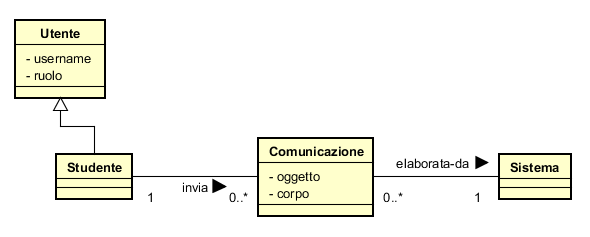
\includegraphics{./images/domain-I1.png}
	\end{center}
	
	I dettagli relativi alle classi sono stati inseriti nel \textbf{Glossario}.
	
	\textbf{Nota:} Non sono state inserite classi o relazioni concettuali relative al login di UC9 in quanto gli elementi trattati non rappresentano oggetti o collegamenti reali, riguardanti il business di uCOM. Questo criterio sarà applicato anche nelle prossime iterazioni.
	
	\newpage
	
	\section{Diagrammi di sequenza di sistema e contratti delle operazioni}
	
	I diagrammi di sequenza di sistema mostrano gli eventi di I/O del sistema \textit{uCOM}, descrivendo in maniera chiara le interazioni tra attori e sistema.
	
	\subsection{UC4: Invia comunicazione}
	\begin{center}
		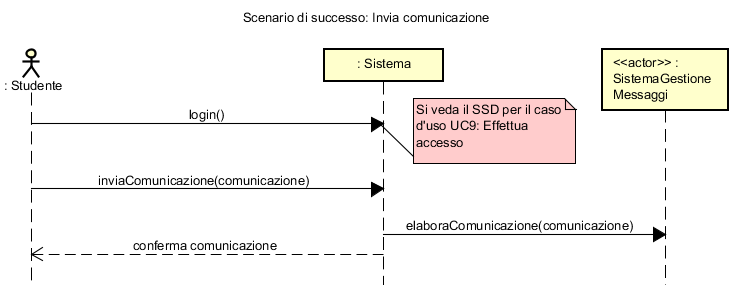
\includegraphics{./images/SSD_UC4.png}
	\end{center}
	
	\newpage	
		
	\subsection{UC9: Effettua accesso}
	
	\begin{center}
		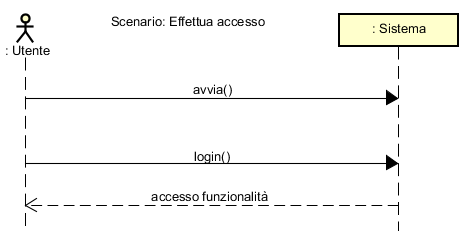
\includegraphics{./images/SSD_UC9.png}
	\end{center}

		%%%%%%% CONTRATTI
	
	\noindent\fbox{%
		\parbox{\textwidth}{%
			\large \textbf{Contratto CO1: login}\\
			
			\normalsize
			\textbf{Operazione:} \quad \quad login()\\
			\textbf{Riferimenti:} \quad \quad Caso d'uso: Effettua accesso\\
			\textbf{Pre-condizioni:} \quad Il Sistema è stato avviato\\
			\textbf{Post-condizioni:} \quad - Un'istanza di Utente u viene creata\\
			.\quad\quad\quad\quad\quad\quad\quad\quad\quad - Il Sistema viene associato all'istanza u \\
			.\quad\quad\quad\quad\quad\quad\quad\quad\quad - Il \textit{ruolo} di u viene associato al Sistema
		}%
	}
	
	
	
	%%%%%%%%%%%% PROGETTAZIONE
	\newpage
	
	
	\section{Diagrammi di sequenza}
	
	I diagrammi di sequenza permettono di iniziare a progettare il software, partendo dall'analisi già effettuata. Essi mettono in evidenza le interazioni tra entità che sono già ottime candidate per diventari classi della programmazione orientata ad oggetti.
	
	\subsection{UC4: Invia comunicazione}
	\begin{center}
		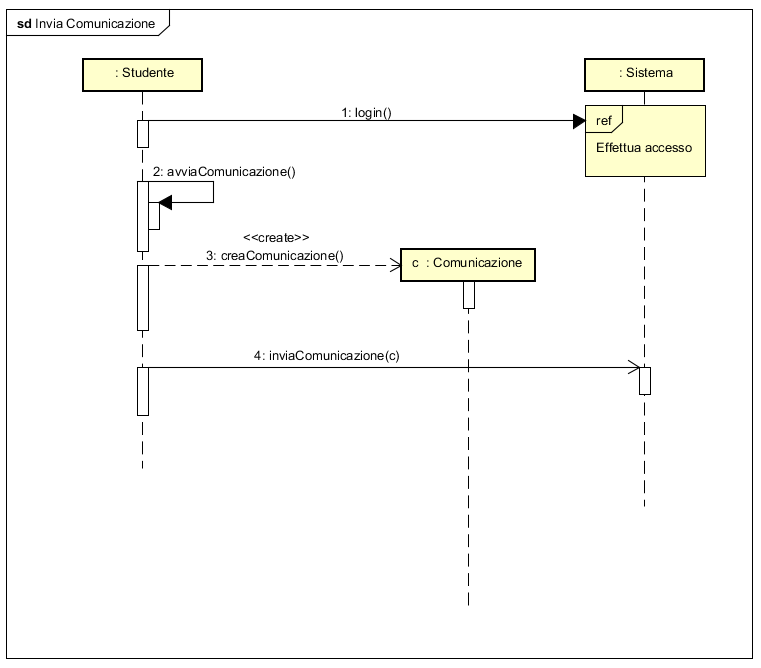
\includegraphics{./images/InviaComunicazione.png}
	\end{center}
	
	\subsection{UC4: Elabora comunicazione}
	\begin{center}
		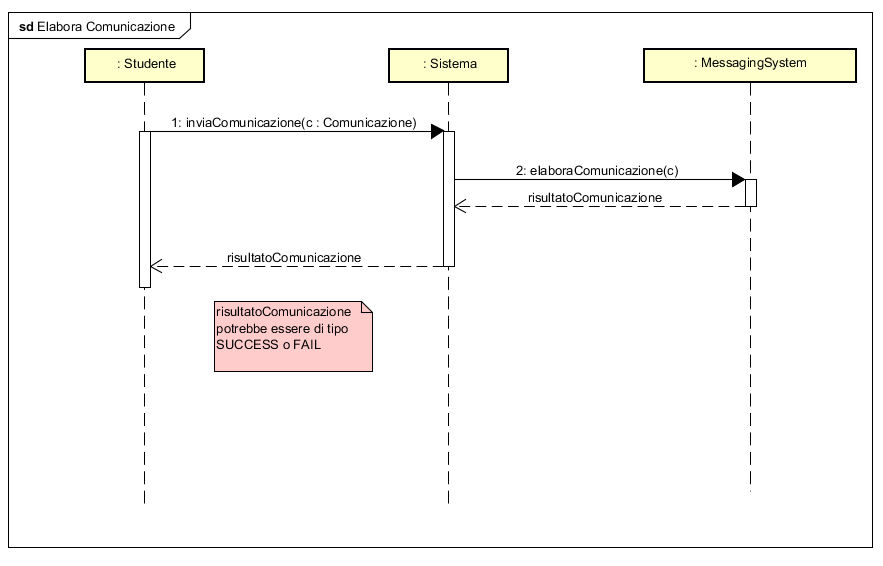
\includegraphics[scale = 0.8]{./images/ElaboraComunicazione.png}
	\end{center}
	
	\subsection{UC9: Effettua accesso}
	\begin{center}
		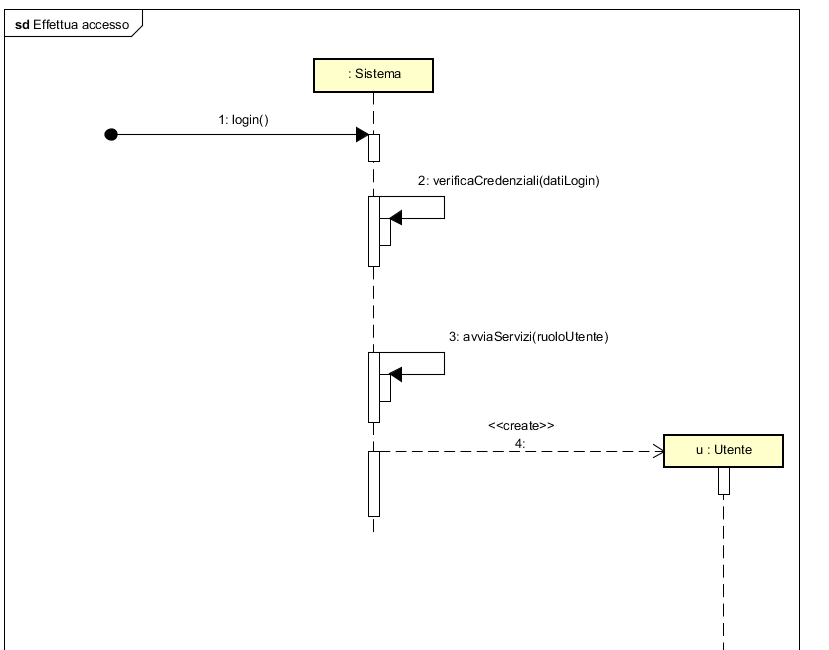
\includegraphics{./images/EffettuaAccesso.png}
	\end{center}
	
	\newpage
	
	\section{Diagrammi delle classi e implementazione}
	I \textit{Diagrammi di sequenza} forniscono una visione dinamica di quanto accade per ciascuna operazione di sistema. Il \textit{Diagramma delle classi} fornisce invece una visione degli aspetti statici, fornendo lo strumento della progettazione più vicino all'implementazione software.
	
	Il Diagramma delle classi che segue è il risultato di un processo di raffinazione, ottenuto applicando pattern GRASP e alcuni Design Pattern [GOF], a partire dagli elaborati dell'analisi e della progettazione finora svolte.
	
	La sua stesura è avvenuta in maniera quasi parallela all'implementazione software, per evidenziare fin da subito i punti critici e le difficoltà nella traduzione del diagramma in codice Java.	
	
	\begin{center}
		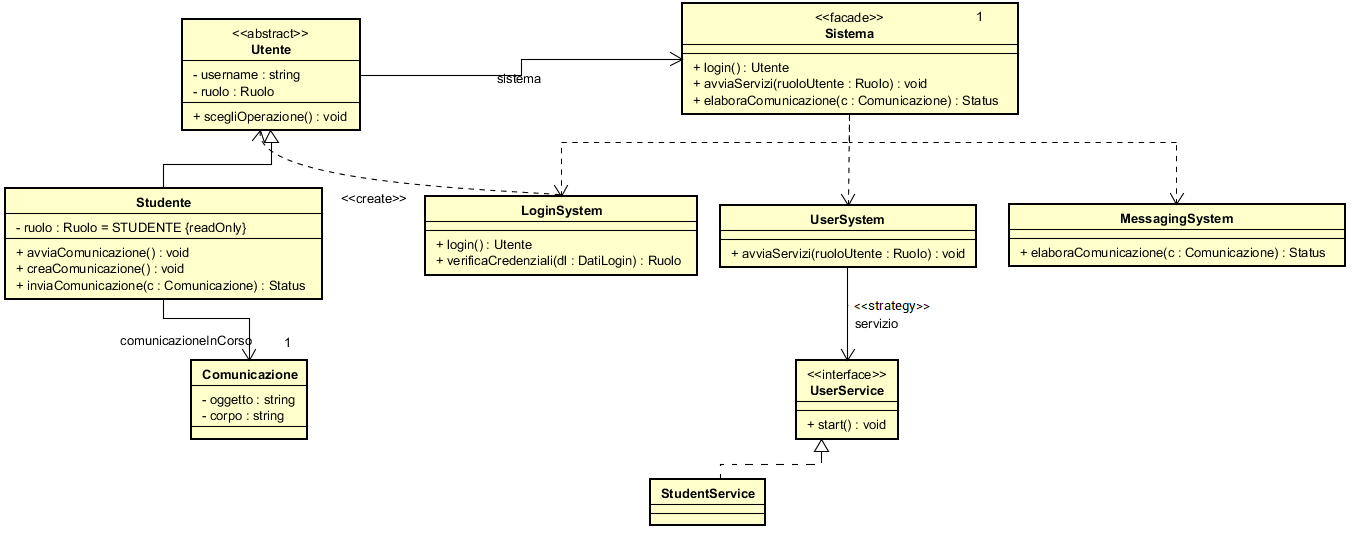
\includegraphics[scale= 0.6]{./images/DCD-I1.png}
	\end{center}

	Sono stati adoperati i seguenti Design Pattern:
	\begin{itemize}
		\item Facade
		\item Singleton
		\item Strategy
	\end{itemize}
	
	Il Sistema, in quanto \textit{Singleton}, possiede un'unica istanza con accesso globale. Su di esso è stato applicato il pattern \textit{Facade} per fornire un'interfaccia unificata per tutti i  sottosistemi di funzioni, accessibile dalle classi degli Utenti, senza aumentare a dismisura la complessità della classe di Sistema. L'applicazione di questo pattern ha permesso di diminuire l'accoppiamento (\textit{Low Coupling}) tra Utenti e sottosistemi, fornendo un \textit{Controller} per tutte le interazioni Utente-Sistema.
	
	Il pattern \textit{Strategy} è utilizzato nel contesto dell'UserService, interfaccia le cui classi concrete hanno il compito di mettere a disposizione dell'utente le funzionalità che gli spettano. Il suo comportamento varia proprio in base al Ruolo dell'utente, definito al momento dell'avvio dei servizi.
	
	Oltre a sviluppare tutte le classi del Diagramma sono state poste le basi per una UI flessibile (al momento funzionante da riga di comando, ma facilmente sostituibile con una GUI) e sono state implementate alcune classi utili per garantire consistenza nell'uso di Nomi e costanti (Status) all'interno del software.
	
	\newpage
	
	%%%%%%%%%%%% TESTING
	
	\section{Testing}
	
	Durante questa iterazione sono state implementate funzionalità di base che corrispondono solo parzialmente a situazioni reali.
	
	Alcuni test funzionali sono stati scritti, per il \textit{LoginSystem} e il \textit{MessagingSystem}, ma venendo restituiti valori di default dalle funzioni testate (senza applicare alcun tipo di condizione o verifica realistica) l'utilità di tali test è pressoché nulla.
	
	Tuttavia pensare a come testare il software è stato utile ad individuare alcune funzioni che andrebbero rese testabili più facilmente - come \textit{creaComunicazione} nella classe \textit{Studente} -, e a pensare a come testare eventuali errori nelle funzioni che restituiscono \textit{void} - si potrebbero creare delle eccezioni adhoc.
	
	Nelle prossime iterazioni verrà effettuato un refactoring di alcune funzioni per renderle testabili, verranno create eccezioni per la segnalazione degli errori e saranno implementati nuovi test, non appena l'implementazione sarà tale da poter testare nuovi scenari, o versioni più complete degli scenari attuali.
	
	Tutti i test per \textit{uCOM} sono stati scritti, e saranno prodotti anche nelle prossime iterazioni, utilizzando il framework \textit{JUnit 5}.
	
	
	
\end{document}